\documentclass[oneside,a4paper,11pt,explicit]{book}
\usepackage[utf8]{inputenc}
\usepackage{icecream}
\usepackage[english]{babel}
\addto\captionsenglish{\renewcommand{\chaptername}{}}
\usepackage[accsupp]{axessibility}  % improves PDF readability for those with disabilities.
\usepackage[colorlinks = true,urlcolor  = blue,linkcolor = blue]{hyperref}
\usepackage{setspace}
\usepackage{listings}
\usepackage[most]{tcolorbox}
\usepackage{minitoc}
\usepackage{multicol}


\renewcommand{\mtifont}{\large\sffamily}
\renewcommand{\mtcfont}{\small\sffamily}
\renewcommand{\mtcSfont}{\small\sffamily}
\renewcommand{\mtcSSfont}{\small\sffamily}
\renewcommand{\mtcSSSfont}{\small\sffamily}
\mtcsetpagenumbers{minitoc}{off} % turn off page numbering in minitocs
\addto{\captionsenglish}{% Making babel aware of special titles
	\renewcommand{\mtctitle}{Quick Links To Sections}
}
\setlength{\fboxrule}{5pt}
\setlength{\fboxsep}{4pt}

\definecolor{IceCreamLeaf}{rgb}{0.4, 0.639215686274, 0.4}
\definecolor{IceCreamOrbit}{rgb}{0.803921568627451, 0.3607843137254902, 0.3607843137254902}

\title{I.C.E.C.R.E.A.M. Tutorials}
\subtitle{\small Observing Earth from Above (Env 329) - Fall 2023  \\
	\small Schmid College of Science and Technology, Chapman University}
\date{\today}

%% DOCUMENT
\setstretch{1.25}
\makeatletter
\begin{document}

\setcounter{tocdepth}{3}
\setcounter{minitocdepth}{3}
\dominitoc
%\tableofcontents

\setcounter{chapter}{9} %Insert (Tutorial Number-1) Here; example for tutorial 4, enter 3

\chapter{Raster Math} %Enter Tutorial Name Here

\vspace{-2em}

\minitoc

\hrule

\vspace{1em}

\begin{tcolorbox}[enhanced,frame style image=blueshade.png,
	opacityback=0.75,opacitybacktitle=0.25,
	colback=blue!5!white,colframe=blue!75!black,title={\Large \textbf{Objectives:}}]
	\large
	\begin{enumerate}
		\item Understand and practice the principles of raster math. 
		\item Apply the results of raster math to a new raster layer and make a map.
	\end{enumerate}
\end{tcolorbox}

\clearpage

%%%%%%%%%%%%%%%%%%%%%%%%%%%%%%%%%% Change Header to Have a Smaller Logo for Remainder of the Document
\fancyhead{}
\fancyhead[C]{\begin{tikzpicture}[overlay, remember picture]
		\fill[Blue2] (current page.north west) rectangle ($(current page.north east)+(0,-1in)$);
		\node[anchor=north west, text=white, font=\Large, minimum size=1in, inner xsep=5mm, align=left] at (current page.north west) {\bf{\MakeUppercase{\@title}}\\\@subtitle};
		\node[anchor=north east, minimum size=1in, inner xsep=5mm] at (current page.north east) {\includegraphics[scale=.125]{ICECREAM_Logo.png}};\end{tikzpicture}}
%%%%%%%%%%%%%%%%%%%%%%%%%%%%%%%%%%

\section{Raster Math Using QGIS Cell Statistics}

Thus far, we have focused on creating maps that represent a single point in time. However, there are many instances where you may want to study multiple points in time. For example, you may want to study the average land surface temperature of a location for the month of July. Or, you may want to study the difference in Evaporative Stress between the months of August and September. 

Or, if you want to study the summer land surface temperature in Mexico City, you would request data from all summer months in A$\rho\rho$EEARS. In return, A$\rho\rho$EEARS would provide 5-10 GeoTIFF files for each month, so you would have to make many maps. This would force your audience to envision how these maps show the average temperature changes over the summer, which would be very challenging. And it would be very time-consuming! 

\vspace{.5em}

There is a better way. QGIS has tools to perform mathematical operations and create a new raster layer of the results. For example, if we have two rasters of the same location and both represent the same type of data (e.g., temperature), we can subtract one from another to produce a new raster of their difference. 

\begin{tcolorbox}[enhanced jigsaw,breakable,pad at break*=1mm,
  colback=yellow!5!white,colframe=IceCreamLeaf,title=An Introduction to Raster Math]

    Raster math requires that you have the same map extent and pixel size (i.e., two or more overlapping maps with the same data resolution). The same mathematical operation (e.g., addition, subtraction, averaging) is then carried out on each pixel. 

    An example of raster subtraction:
 
    \vspace{.5em}

    \centerline{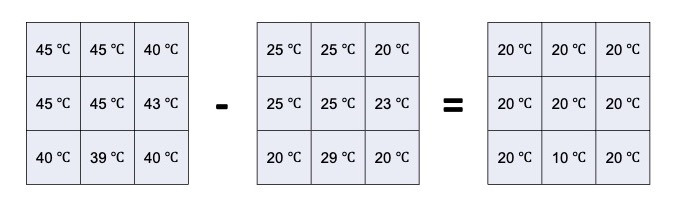
\includegraphics[width=\textwidth]{RasterMathExample.png}}

    \vspace{.5em}

However, if the two rasters have different extents (e.g., one is a map of Nevada and the other is a map of Nevada and California), then the process will fail. 

   An example of a mismatched extent:
   
    \vspace{.5em}

    \centerline{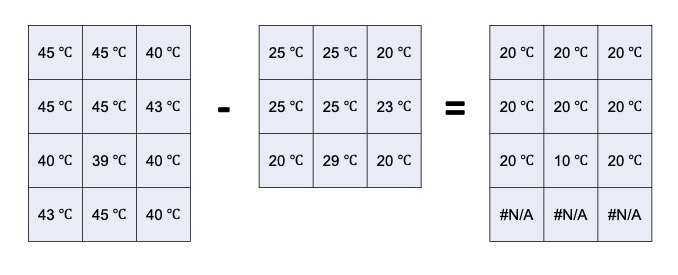
\includegraphics[width=\textwidth]{RasterMath-MismatchedExtent.png}}

    \vspace{.5em}
     
    Similarly, if the two rasters have the same extents but different pixel sizes (e.g., one is a map where each pixel is 50 sq. m and a second where each pixel is 100 sq. m, the the process will fail. 

   An example of a mismatched resolution:
   
    \vspace{.5em}

    \centerline{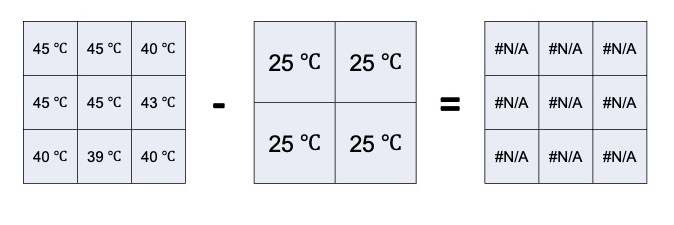
\includegraphics[width=\textwidth]{resolution.png}}

    \vspace{.5em}
 
    Finally, if for some reason the rasters have different projections (the way in which data is represented in two dimensions), then this can cause both the extent and pixel size to differ. 

     \vspace{.25em}
 
    Raster math can be challenging when you get started, but once you get the hang of it, you will realize that it is a very powerful tool! 

\end{tcolorbox}

\vspace{.5em}

1. Open QGIS and start a new project by selecting the \textit{Project} menu, then \textit{New}.

2. To add a basemap, find the \textit{HCMGIS} menu bar, select \textit{Basemap}, then pick your preferred map. For today's map, we recommend using \textit{Google Satellite}. Note that clicking on a basemap type automatically adds a new layer to your map, as seen in the layer browser window.

3.Load in this GeoJSON file for Mexico City : (\href{https://jeremydforsythe.github.io/icecream-tutorials/Tutorial8_ESI/MexicoCityPolygon/MexicoCity.geojson}{\small MexicoCity.geojson})

\vspace{.5em}

\centerline{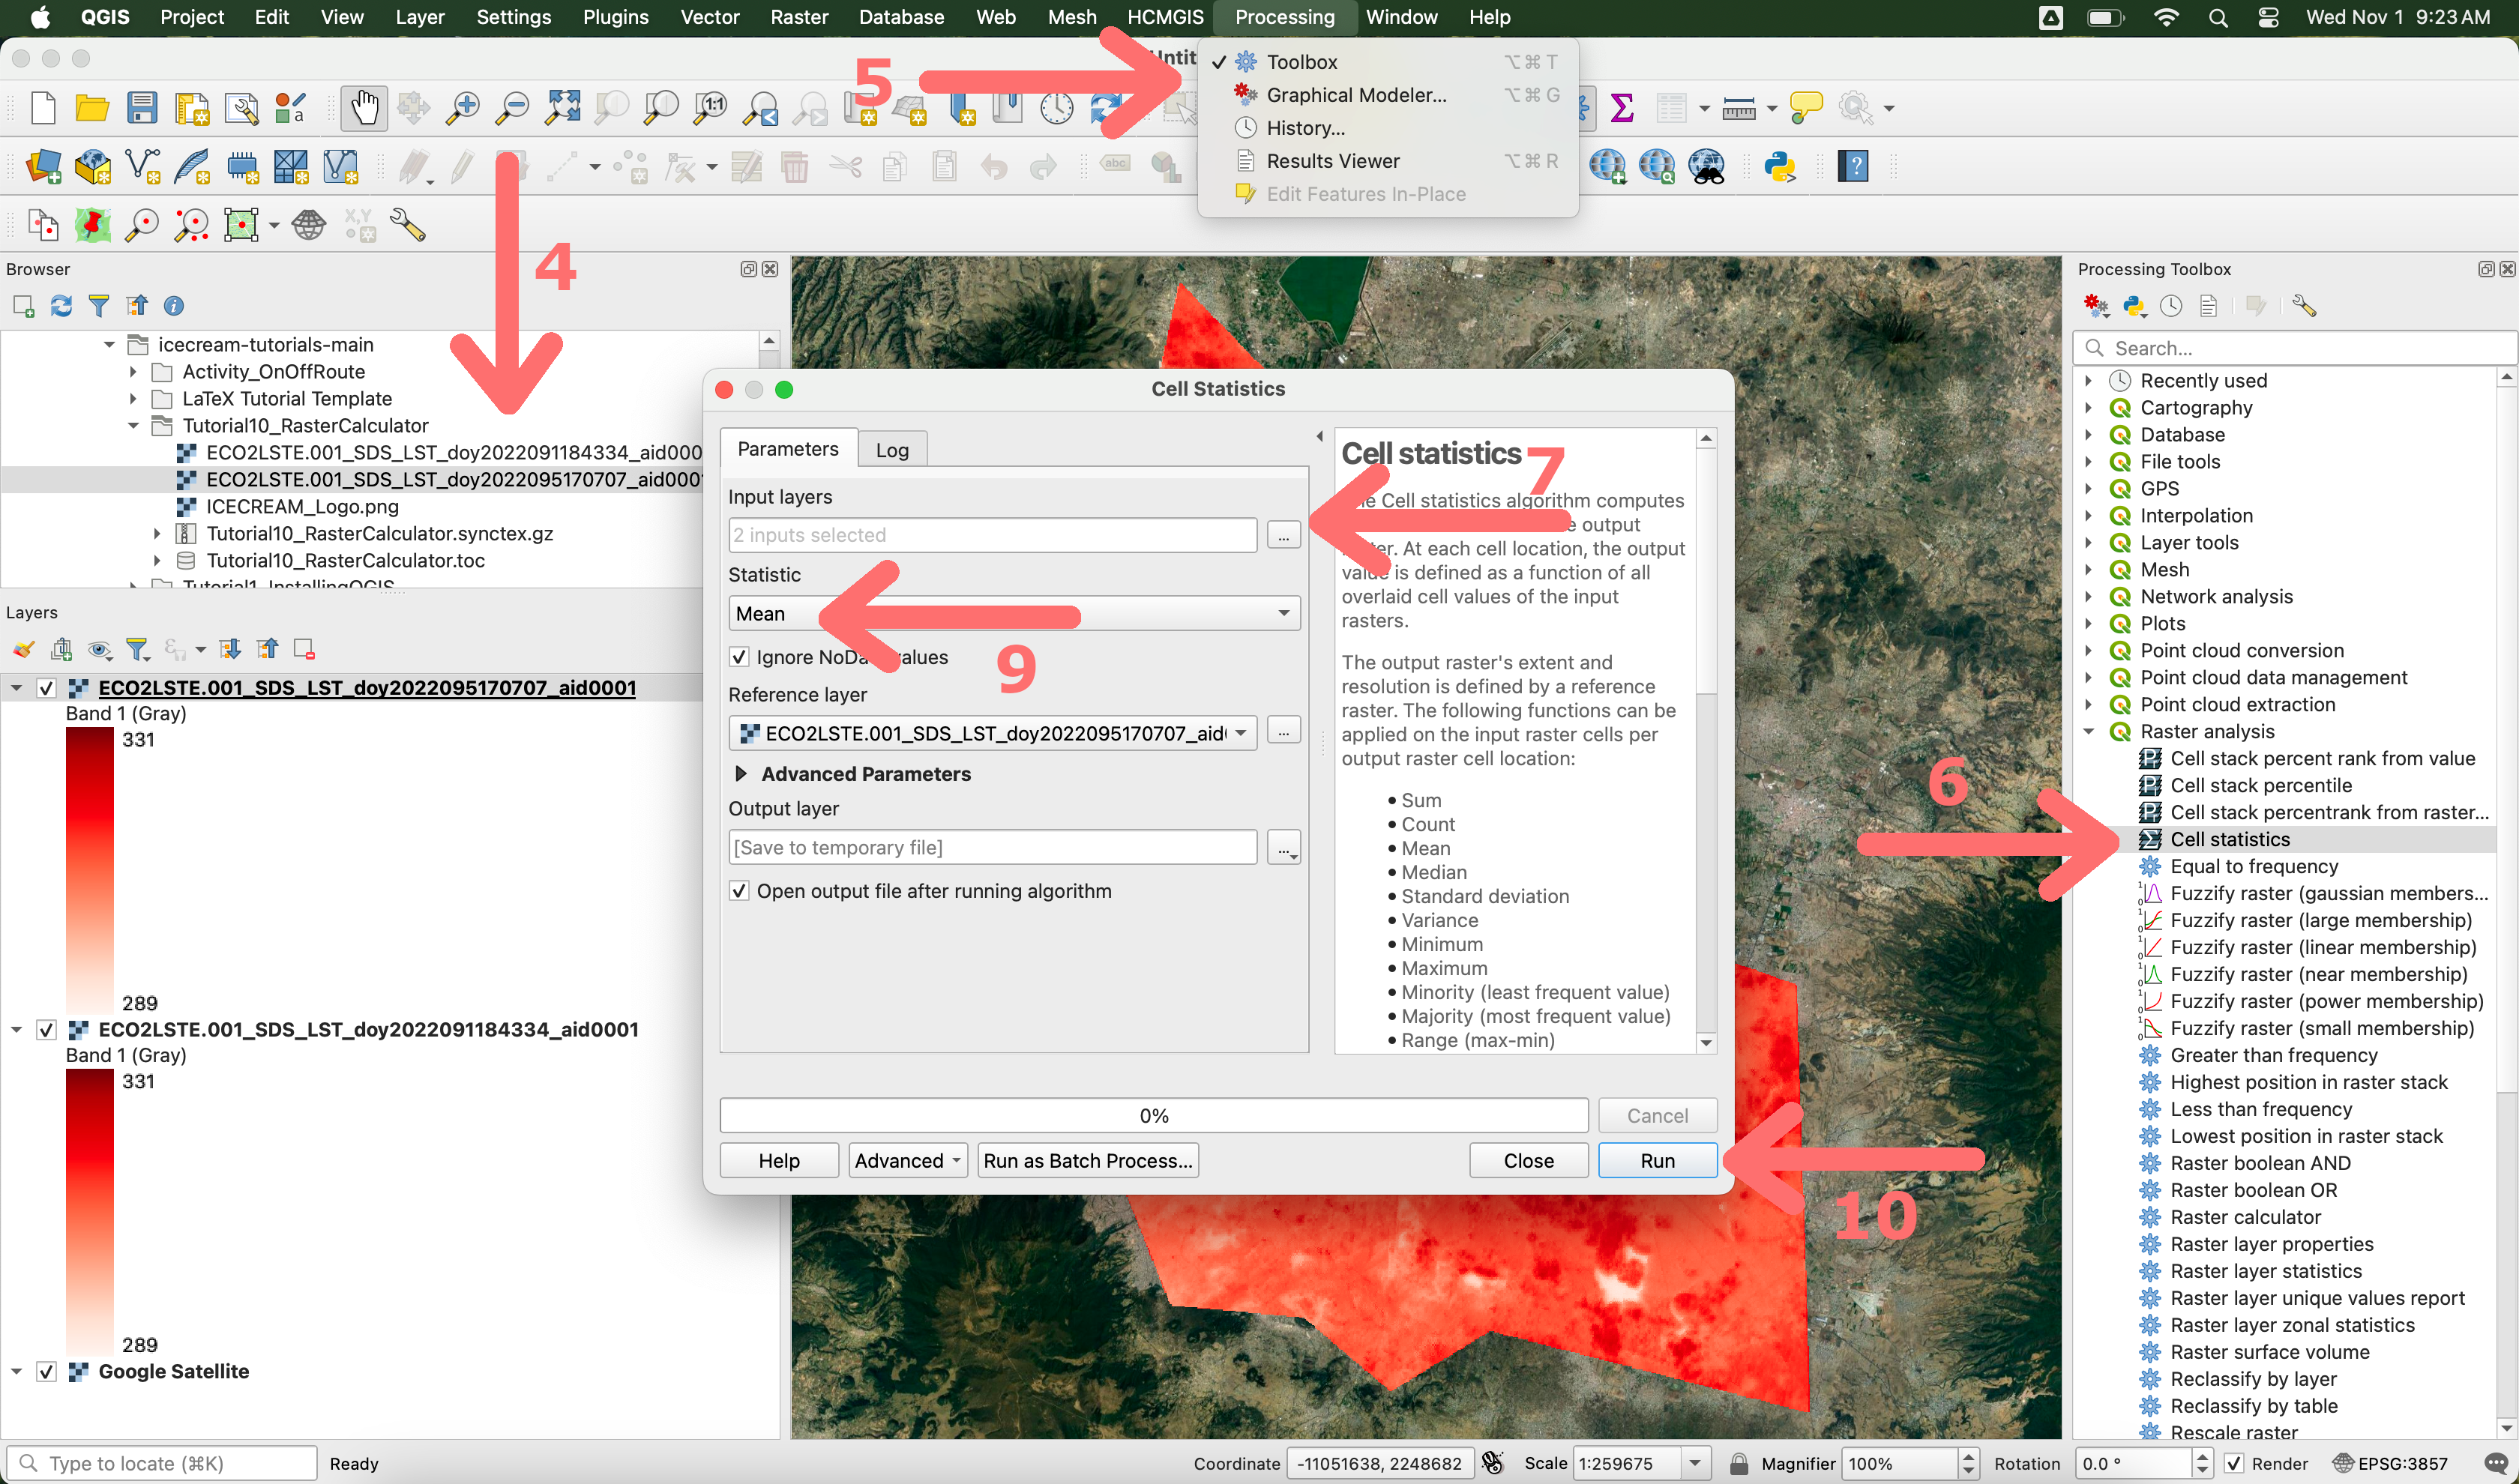
\includegraphics[width=\textwidth]{CellStatistics.png}}

\vspace{.5em}

4. Download these GeoTIFF files that we have pre-selected for you. They are the ECOSTRESS land surface temperatures for Mexico City from April 2022. Save them somewhere that you can remember and then add them as layers in QGIS. 

\begin{itemize}
    \item \href{https://jeremydforsythe.github.io/icecream-tutorials/Tutorial10_RasterCalculator/ECO2LSTE.001_SDS_LST_doy2022091184334_aid0001.tif}{\small ECO2LSTE.001\_SDS\_LST\_doy2022091184334\_aid0001.tif}
    \item \href{https://jeremydforsythe.github.io/icecream-tutorials/Tutorial10_RasterCalculator/ECO2LSTE.001_SDS_LST_doy2022091184334_aid0001.tif}{\small ECO2LSTE.001\_SDS\_LST\_doy2022091184334\_aid0001.tif}
\end{itemize}

\vspace{.5em}

\centerline{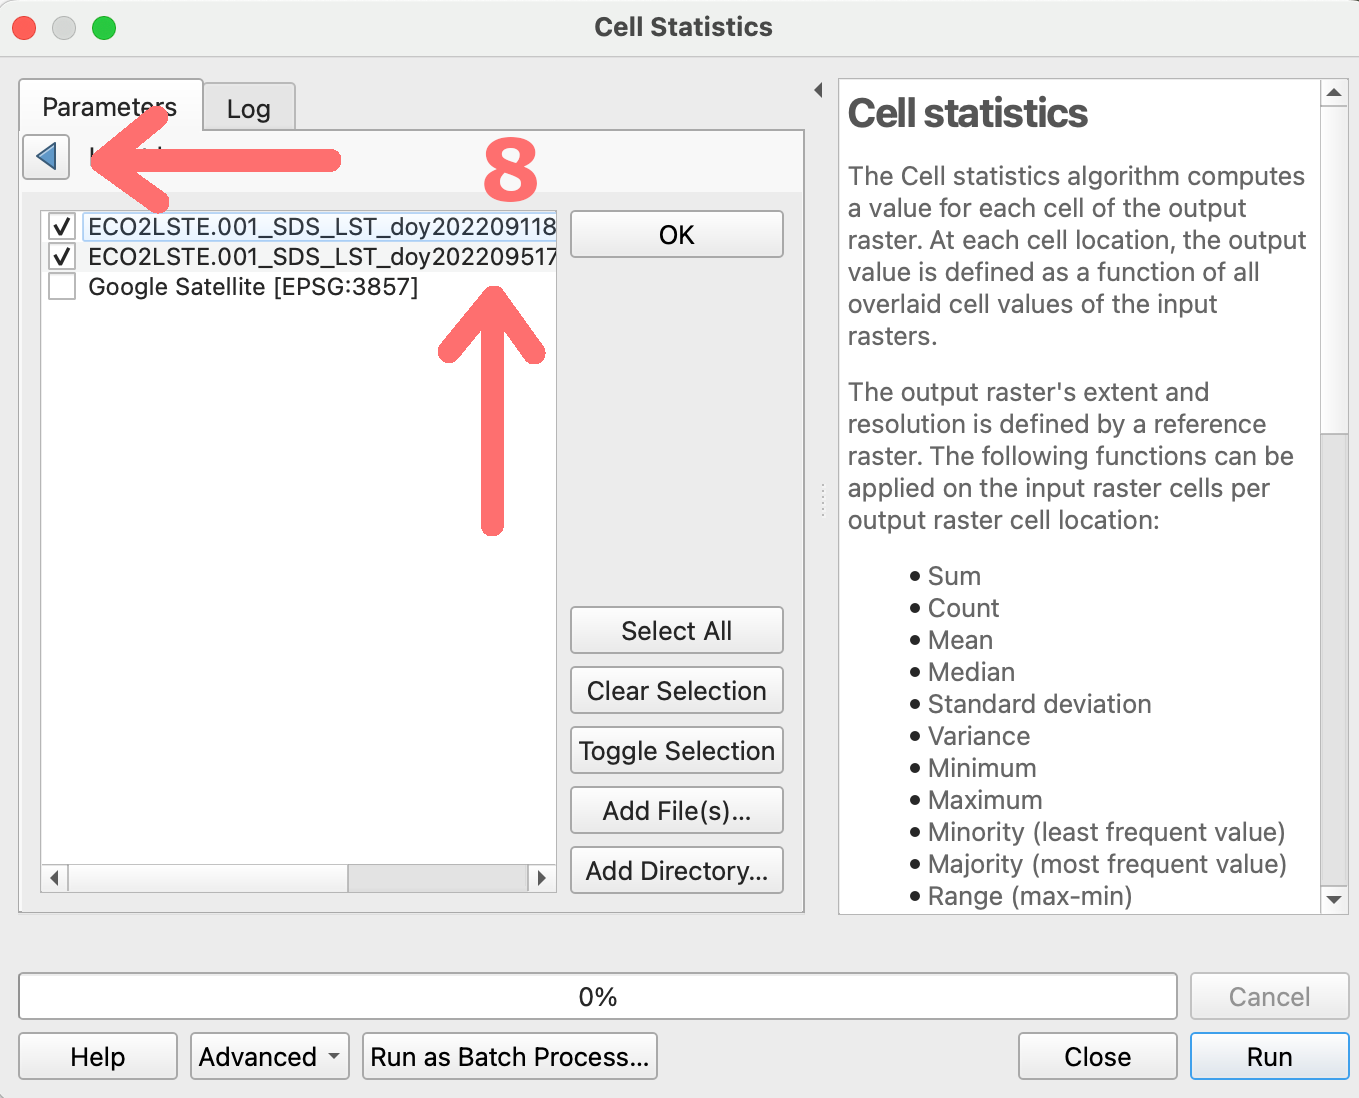
\includegraphics[width=.6\textwidth]{CellSelect.png}}

\vspace{.5em}

5. From the QGIS top menu bar select \textit{Processing}, then click \textit{Toolbox}.

6. From there find the folder \textit{Raster Analysis} and double click on \textit{Cell Statistics}.

7. Click the ``...'' button next to the \textit{Input Layers} dialog box. 

8. Select the layers you want to do raster math on, in this case the two Mexico City GeoTIFF files we provided.

9. The \textit{Statistics} box has the options to choose what type of raster math you want to calculate. Today let's use ``Mean'' to take the average temperature of our two GeoTIFFs. 

10. Click the \textit{Run} button.

\vspace{.5em}

\centerline{\includegraphics[width=\textwidth]{CellOutput.png}}

\vspace{.5em}

11. You now have a new layer that is the mean land surface temperature of the two GeoTIFFs for Mexico City.

12. To visualize this mean, deselect the other two layers. You can now change the color symbology and produce complete maps with this new layer. 

\kulbox{\textbf{NOTE:} This new layer can be exported by right-clicking (ctrl-click on Mac) as a GeoTIFF and clicking \textit{Save as...}. You can even use these output layers to create new layers with the same process. Maybe you want to look at the difference between the mean land surface temperatures of August 2022 and August 2023 for Death Valley. You can string together some raster analysis to acheive this goal!}

\begin{tcolorbox}[colback=yellow!5!white,colframe=IceCreamOrbit,title= \vspace{.2em} \Large Map of the Week Assignments]
	\addcontentsline{toc}{section}{Map of the Week Assignments}
	\large
	\begin{enumerate}
		\item Submit a map for Mexico City with the averages of land surface temperature for the two files we provided. 
		\item Include a one-paragraph interpretation of the process of building your map and the results.  
	\end{enumerate}
	Submit these assignments via Canvas before the next class.
\end{tcolorbox}

\begin{tcolorbox}[colback=yellow!5!white,title=\textbf{Datafiles}]
	\addcontentsline{toc}{section}{Datafiles}
	\large
	In case you encountered any issues with the A$\rho\rho$EEARS database, here are copies of the ECOSTRESS GeoTIFF file for Mexico City:

    \begin{enumerate}
        \item \href{https://jeremydforsythe.github.io/icecream-tutorials/Tutorial10_RasterCalculator/ECO2LSTE.001_SDS_LST_doy2022091184334_aid0001.tif}{\small ECO2LSTE.001\_SDS\_LST\_doy2022091184334\_aid0001.tif}
        \item \href{https://jeremydforsythe.github.io/icecream-tutorials/Tutorial10_RasterCalculator/ECO2LSTE.001_SDS_LST_doy2022091184334_aid0001.tif}{\small ECO2LSTE.001\_SDS\_LST\_doy2022091184334\_aid0001.tif}
        \item And my Mexico City shapefile: \href{https://jeremydforsythe.github.io/icecream-tutorials/Tutorial8_ESI/MexicoCityPolygon/MexicoCity.geojson}{\small MexicoCity.geojson}
    \end{enumerate}
\end{tcolorbox}

%%%%%%%%%%%%%%%%%%%%%%%%%%%%%%%%%%%%%%%%%%%%%%%%%%%%%%%%%%%%%%%%%%%%%%%%%%%%%%%%%%% End of Document
%\vfill

\hrule

\vspace{1em}

\small \textbf{Recommended Citation:} Forsythe, J.D., G.R. Goldsmith, and J.B. Fisher. 2023. Observing Earth from Above Tutorials. Chapman University. \url{https://jeremydforsythe.github.io/icecream-tutorials/}

\vspace{1em}

This work is supported by funding from NASA ECOSTRESS Mission Grant \#80NSSC23K0309 (I.C.E. C.R.E.A.M.: Integrating Communication of ECOSTRESS Into Community Research, Education, Applications, and Media).

\end{document}
